\chapter{Formalising ZKBoo}
\label{ch:formal_zkboo}
In this chapter we show how to use our previous formalisations of
$\Sigma$-Protocols and commitment schemes to formalise the ZKBoo protocol
introduced in the previous chapter.
Here we will shown how to instantiate ZKBoo with our $\Sigma$-Protocol
formalisation and then show how we can use our formalisation of commitment
protocols to prove the security of ZKBoo.

The goal of formalising ZKBoo is two-fold. First, we show that our previous
formalisations are indeed applicable to larger protocols. Second, we aim to
gather insight into how \easycrypt\ can help in formalising protocols larger
than the usual toy examples like El-Gamal and Schnorr.

\paragraph{Outline}
First, in section \ref{sec:arith_circuits} we find develop a formalisation of
arithmetic circuits within \easycrypt\ , which allows us the reason about
evaluating the circuit to a value and guide the formalisation of the
decompostion. Next, in section \ref{sec:decomposition} we formalise the
(2,3)-Decomposition of arithmetic circuits as defined in section
\ref{sec:arith_circuits}.
This ultimately leads to section \ref{sec:formal_zkboo} where we use the
formalisation of arithmetic circuits and their (2,3)-Decomposition to
instantiate ZKBoo as a $\Sigma$-Protocol and then prove its security.


\begin{figure}[ht]
  \centering
  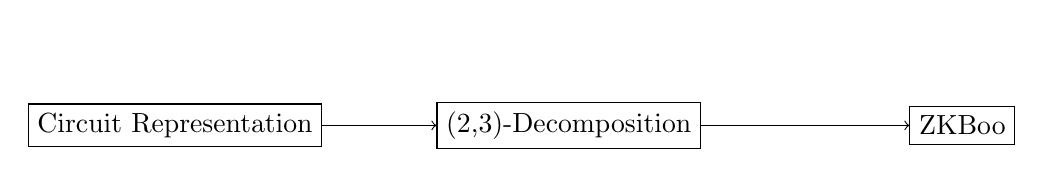
\begin{tikzpicture}
      \node[draw] at (-20,.3) (a) {Circuit Representation};
      \node[draw] at (-15,.3) (b) {(2,3)-Decomposition};
      \node[draw] at (-10,.3) (c) {ZKBoo};

      % draw edges
      \draw[->] (a) -- node[midway,above,yshift=1cm] {} (b);
      \draw[->] (b) -- node[midway,above] {} (c);
  \end{tikzpicture}
  \caption{\label{fig:outline_zkboo} Outline of ZKBoo formalisation}
\end{figure}

\paragraph{Preliminary notation}
Throughout this chapter use the letter $e$ to denote an integer in \{1,2,3\}.
Moreover, we define arithmetic on $e$ such that $3+1 = 1$.

To refer to the i'th index of a list $w$ we use the notation $w[i]$.

\section{Formalising Arithmetic circuits}
\label{sec:arith_circuits}
In this section we will introduce the concept of arithmetic circuits and how they
can be represented. Primarily we recall the usual definition of circuits as
graph and discuss how to evaluate circuits programmatically. From this we
introduce a number of restrictions to our formalisation which makes their easier
to work with, whilst still being expressive enough to use in the ZKBoo protocol.
Based on these restrictions we then formulate an alternative representation for
arithmetic circuits and give a number of key definitions, which are needed for
reasoning about the structure of a circuit and the evaluation of circuits.

\subsection{Representing an arithmetic circuit}
\label{subsec:arith-representation}
An arithmetic circuit is in its most general form express a function $\phi$ over some
arbitrary field $\mathbb{Z}_{q}$, where $\phi : \mathbb{Z}_{q}^{k} \rightarrow \mathbb{Z}_{q}^{l}$

To express arbitrary (Arithmetic) computations in a ring of finite field we
use the following four gates, addition by constant (ADDC), multiplication by constant
(MULTC), addition of two wires (ADD), and multiplication of two wires (MULT).

The goal of this section is to formulate a representation of the function
$\phi$, which only depends on the aforementioned gate types to perform
computations. Before doing so, however, we start by stating a number of
simplifying assumptions about our arithmetic circuits. First, we only allow the
circuit to have one input value and one output value, in other words:
$k = l = 1$ in the definition of $\phi$.
This assumption exists pure to make it easier to reason about the inputs and
output of the function. The formalisation in this section could be altered to
allow for arbitrary inputs with minor alterations, which we will discuss later.
\todo{Discuss this later}

Based on these simplifying assumptions we can now recall the graph
representation of a circuit:
\begin{definition}[Arithmetic Circuit]
  \label{def:arith_circuit}
  An Arithmetic circuit is a graph C = (W, G) where W is the internal
  wires between the gates and G is the set of gates within the circuit. Then,
  we let $i \in G$ be first gate of the circuit, i.e. its only input and $o \in G$ be the output
  gate, for which there must exists a path from i to o in W.
  Specifically, o is a gate with only one in-going wire and no out-going wire.
  The means that the value of the circuit can be read by reading the value of
  the in-going wire to o.

  \todo{Define in- and out-wires?}

  Finally, for all gates $g \in G$ there must exists path in W from i to o going
  through g,
  since if this was not the case, the gate does not contribute the output of the
  gates and can therefore be removed from the graph without changing the
  semantic meaning of the circuit.
\end{definition}

To define evaluation of a circuit we would then need compute the value of the
in-wire of o, but this can only be done if we have computed all other wires in
the circuit. Moreover, the value of the out-wires of a given gate, g, can only
be computed if all in-wires of g has already been computed to a value. It is
clear from this that we need to define an order of evaluation, such that we only
try to compute the out-wire of a gate if we know that all in-wires has been computed.

To define the order of evaluation we follow the work of \cite{Yao} and introducing an alternative
representation of Arithmetic circuits, which naturally gives us a well-defined
evaluation order:

\begin{definition}[List representation of arithmetic circuits]
  Given an arithmetic circuit C as defined by definition \ref{def:arith_circuit}
  we define the list representation of C as computing a linear ordering, O, of
  G, which gives each gate in G an unique index.
  \todo{Why do we remove i and o?}
  We then let the list representation $C_{L}$ be defined as:
  \[
    C_{L}[j] = Enc(O( G \setminus \{i\})[j], W)
  \]

  Where $Enc : gate \rightarrow W \rightarrow \text{encoded gate}$, is a function
  taking as input a gate and the wires of the circuit and produces an encoded
  gate.
  The encoded gate contains type information about gate but also stores the
  indexes (From the linear ordering) of the gates, whose out-going wires are the
  in-going wires of the gate.
  The type declaration of the encoded gates can be seen in figure \ref{lst:gate_types}.
\end{definition}

\todo{Tikz example showing the two representations}

\todo{This representation does not allows for optimisations like parallel computations}

\paragraph{Linear ordering}
A linear ordering O is a function that when applied to G assigns a unique
index to each gate in G.
One example of such function defining a linear ordering is a breadth-first
search, where each gate in the circuit graph is labelled according to at which
time the BFS reached the gate.
This labelling would start at gate $i$ and end at $o$.

A special property of the linear ordering induced by a BFS labelling is that a
gate can only be visited when all nodes that the gates computation can depend on
has already been visited. This ensure that for a node indexed $i$ it only
depends on out-wires of nodes with index less-than $i$.

This ordering allows us to convert the graph representation into a list
representation, where the gate at index $i$ is the node with index $i$ by the
linear ordering. However, since the gates $i$ performs no computation and only
exists to add the input value to the graph we exclude it from the list
representation, and shift every index one down.

\paragraph{Encoded gates}
A gate is then a type, which defined its operation along
with a tuple $(l,r)$ where $l$ is the index of left input wire and $r$ is the
index of the right input wire. In the case of unary gates like ADDC and MULTC
the tuple is $(l, c)$ where l is the input wire and $c$ is the constant used in
the computation.

But we need to encode W into this list. To do this we encode the information
about input wires into the types of the gates themselves, as seen in figure
\ref{lst:gate_types}.

\begin{lstlisting}[float,label=lst:gate_types,caption=Type declaration of gates]
type encoded_gate = [
  | ADDC of (int * int)
  | MULTC of (int * int)
  | MULT of (int * int)
  | ADD of (int * int)
].
\end{lstlisting}
\vspace{2mm}
\noindent
One important aspect of the list representation of circuits is that it allows
us to easily define an evaluation order, where we are ensure that we are not
computing the value of a gate before the previous gates has been computed. To
capture this notion of a valid evaluation order we give the following definition:

\todo{Define notation for list indexing?}

\begin{definition}[Valid circuit]
  \label{def:decomp:valid_circuit}
  An arithmetic circuit in list representation $C_{L}$ is valid if for every
  entry $i$ in the list it holds that:
    \begin{itemize}
      \item C[i] is a gate type
      \item the input wires of C[i] have index less than $i$.
      \item the input wires of C[i] have index greater than or equals to $0$.
    \end{itemize}
\end{definition}

\begin{lstlisting}[float,label=lst:circuit_eval,caption=Circuit evaluation function]
op eval_gate (g : gate, s : int list) : int =
  with g = MULT inputs => let (i, j) = inputs in
                          let x = (nth 0 s i) in
                          let y = (nth 0 s j) in x * y
  with g = ADD inputs =>  let (i, j) = inputs in
                          let x = (nth 0 s i) in
                          let y = (nth 0 s j) in x + y
  with g = ADDC inputs => let (i, c) = inputs in
                          let x = (nth 0 s i) in x + c
  with g = MULTC inputs => let (i, c) = inputs in
                          let x = (nth 0 s i) in x * c.

op eval_circuit_aux(c : circuit, s : int list) : int list =
    with c = [] => s
    with c = g :: gs =>
     let r = eval_gate g s in
     eval_circuit_aux gs (rcons s r).

op eval_circuit (c : circuit, s : state) : output =
    last 0 (eval_circuit_aux c s).
\end{lstlisting}

From this representation of circuits as a list of gates, where gates are types,
it is possible to define the semantic meaning of this representation, by
defining the evaluation function, which can be seen in figure \ref{lst:circuit_eval}.
The evaluation is broken into two parts: First we have a function for evaluating
one gate to an intermediate values. Second, we have a procedure for evaluating
the entire circuits which calls the former function.
To evaluate a single gate, we first need to determine which gate it is. This can
be done by utilizing the power of the \easycrypt\ type system, which allows us
to pattern match on the type of the gate as seen in listing \ref{lst:circuit_eval}.

Then, if the circuit is valid the evaluation order is the indexes of the list representation.
We know that if we are computing index $i$ of the circuit, then indices
$[0 \dots i-1]$ have already been computed. Perform the appropriate function
then reduces to looking up the values of the previously computed gates and
applying them to the function appropriate for the type of the gate.

Computing the entire circuit then follows from the same fact, that gates are always
evaluated in the order the appear in the list, and the no gate can depend on
the result of gates, which have a higher index than itself. By continually
performing gate evaluation of the next entry in the list and saving the result
into ``state'' where each index correspond to the computed value of the gate at
that index in the circuit, and the calling recursively on the list with the
first entry removed, then the output of the gate will be in the last entry of
the state, when there are no more gates to compute. Assuming that there is only
one output gate.

\begin{definition}[State of list representation]
  For a list representation of a circuit $C_{L}$ we give the following recursive
  definition of the state:
  \begin{align*}
    \text{state}[0] &= \text{input value} \\
    \text{state}[i>0] &= \texttt{eval\_{gate} } C_{L}[i-1] \; state[i-1]
  \end{align*}

  Here we recall that input gate has been removed from the list representation
  and $C_{L}$[0] is the first non-input gate in the circuit. From this it also
  follows that
  \begin{equation}
    \text{size } \text{state} = \text{size } C_{L} + 1
  \end{equation}
\end{definition}

We then have that any valid circuit c can be compute to a value y as
\texttt{eval\_circuit(c, [input]) = y}. This can also be stated as a probabilistic
procedure as $\Pr{\texttt{eval\_circuit(c, [input])} = y} = 1$.

To reason about functions and procedures about functions we have the following lemma:
\begin{lemma}[Function/Procedure relation]
  \label{lem:func/proc-equiv}
  $\forall$ f, inputs, output: f(inputs) = output $\iff \Pr{f(inputs) = output} = 1$.
\end{lemma}
\begin{proof}
  \hspace{2mm}
  \begin{itemize}
    \item  ``$\Rightarrow$'':
      Trivial
    \item  ``$\Leftarrow$'':
      by contradiction?
  \end{itemize}
\end{proof}

\todo{ZKBoo paper gives no notion of a valid evaluation order - needed for security}

\todo{Graph representation isomorphic to list representation?}


\section{(2,3) Decomposition of circuits}
\label{sec:decomposition}
In this section we ... formalisation based on the description of arithmetic circuits...
\todo{mention MPC}

In its most general form, we can define the decomposition as a procedure taking
as input three views and random tapes, and a circuit and produces three new
views. \todo{rewrite? - Random tapes = set of random choices}
More specifically the decomposition work by incrementally evaluating a gate based on
previously compute views, which yield new shares that can be appended to the
view. This process of evaluating a single gate based on the view of evaluating
the previous gate can then be repeated until all gates have been computed. This
overall idea has been captured in the procedure in figure \ref{lst:decomp_aux},
where it is assumed access to a function eval\_gate, which has signature:
$eval\_gate : circuit \Rightarrow party \Rightarrow (view * view) \Rightarrow (random\_tape * random\_tape) \Rightarrow share$,
\todo{explain eval gate better?}
where $party$ is a integer in $\{1,2,3\}$ that determines which party is
computing the share. \todo{Say that eval gate implements the function in the
  ZKBoo section}

The output of the decomposition can then be defined as summing the last share from each view that has been compute by the aformentioned procedure. More formally the output is:
\begin{equation}
  \text{Output}(w1, w2, w3) = \sum_{i \in \{1,2,3\}} \text{last } w_{i}
\end{equation}


\begin{definition}[Correctness of views]
  \label{def:decomp:valid_view}
  For any three views (list of shares), $w_{1}, w_{2}, w_{3}$, with equal length, we
  say that they contain valid shares of computing a circuit c, if it holds:

  \begin{equation}
    \label{eq:decomp:view:sum}
    \forall 0 \leq i < \text{size } c,
      \sum_{p \in \{1,2,3\}} w_{p}[i] = s[i]
  \end{equation}

  where s is the list of intermediate values produces by calling
  \texttt{eval\_circuit\_aux} in figure \ref{lst:circuit_eval}.

  Additionally a share is only valid, if it has been produced by functions used
  by the decomposition. This property also ensures that the views are consistent wrt. each other. Namely, if $p_{i}$ computes a share $s$ then $s$ is the share that the other parties received from $p_{i}$ during the execution of the protocol.

  \begin{equation}
    \label{eq:decomp:valid}
      \forall 0 \leq i < \text{size
                                                   } c - 1,  w_{e}[i+1] = \texttt{eval\_gate } c[i]\; w_{e} \; w_{e+1}
  \end{equation}

  To express that the views satisfy the above definition we use the notation
  \validviews{c,w1,w2,w3} to express that $w1, w2, w3$ are valid views for the
  decomposition of $c$

\end{definition}


\begin{lstlisting}[float,label=lst:decomp_aux,caption= Incremental decomposition procedure]
  proc compute(c : circuit, w1 w2 w3 : view, k1 k2 k3 : random_tape) = {
    while (c <> []) {
      g = oget (ohead c);
      r1 <$ dinput;
      r2 <$ dinput;
      r3 <$ dinput;
      k1 = (rcons k1 r1);
      k2 = (rcons k2 r2);
      k3 = (rcons k3 r3);
      v1 = eval_gate g 1 w1 w2 k1 k2;
      v2 = eval_gate g 2 w2 w3 k2 k3;
      v3 = eval_gate g 3 w3 w1 k3 k1;
      w1 = (rcons w1 v1);
      w2 = (rcons w2 v2);
      w3 = (rcons w3 v3);
      c = behead c;
    }
    return (k1, k2, k3, w1, w2, w3);
  }
\end{lstlisting}

\paragraph{Handing randomness}
\label{subsec:decomp:randomness}
Looking at compute we see that compute we make three random choices for each gate and then save those choices to some random tapes. These tapes are then returned. They are used to keep track of the random choices made thoughout the protocol, such that views can be verified. For most proof the specific values contained within the random tapes are not imporant, since the random values are only there to cancel eachother out whilst making the shares look randomly distributed.
We therefore omit the random tapes for most procedures and proofs in this section, since they are static?
When the random tapes are imporant for the security we will mentioned how.

The reason for sampling random values at each iteration of the while loop instead of all at once is to be able to reason about the specific random choices made at this time in the computation. This is especially important to be able to relate two procedures running at the same iteration of the while loop...


\subsection{Correctness}
\label{sec:decomp_correct}
Ultimately want to prove:
\begin{lemma}[Decomposition correctness]
  \label{lem:decomposition_correctness}

  \[
    \Pr{\texttt{eval\_circuit(c, [input])} = y} =
    \Pr{\texttt{decomposition(c, [input])} = y}
  \]

  i.e. The output distribution of the two programs are perfectly indistinguishable. From lemma \ref{lem:func/proc-equiv} we have that circuit evaluation always succeeds. This lemma, therefore, also implies that the decomposition always succeeds.
\end{lemma}

To prove the above lemma we first introduce a helper lemma:

\begin{lemma}[Stepping lemma for decomposition]
  \label{lem:decompose_compute_step}
  For any valid circuit c in list representation, it is possible to split the circuit into two parts
  $c_{1}, c_{2}$ where $c = c_{1} ++ c_{2}$ (++ is list concatenation).
  let $w_{1}, w_{2}, w_{3}$ be the resulting views of decomposing $c$ and
  \validviews{c_{1}, w_{1}, w_{2}, w_{3}} and let computing $c_{2}$ with initial
  views $w_{1}, w_{2}, w_{3}$ output views $w'_{1}, w'_{2}, w'_{3}$.
  Then \validviews{c, w'_{1}, w'_{2}, w'_{3}}.

  Alternatively this is stated as:
  \[
    \textbf{Valid}(c_{1}, w_{1}, w_{2}, w_{3})  \implies
    \Pr{ \texttt{compute}(c_{2}, w_{1}, w_{2}, w_{3}) : \textbf{Valid}(c, w'_{1} , w'_{2}, w'_{3}) } = 1
  \]

\end{lemma}
\begin{proof}
  The proof proceeded by induction on the list c.

  \begin{itemize}
    \item Base case $c = []$:
        trivially true since an empty circuit is the identity function.
    \item Induction step $c = c' ++ [g]$:
      \begin{itemize}
        \item Inline definitions to get compute\_stepped
        \item We use to induction hypotheses to compute c' which give us
              \validviews{c_{1}, w_{1}, w_{2}, w_{3}}.
        \item We then need to prove, that we can compute any gate on top of the
          valid views to produce a new set of valid views.
      \end{itemize}
  \end{itemize}

\end{proof}

\begin{proof}[Proof of lemma \ref{lem:decomposition_correctness}]
  By unfolding the definition we are left with proving that the last share from
  each of the views produced by \texttt{compute} are equal to the output of
  evaluating the circuit, which is true by lemma \ref{lem:decompose_compute_step}
\end{proof}

\todo{Our formalisation differs by imposing stricter restrictions on the shares computed...}


\subsection{2-Privacy}
\label{sec:decomp_privacy}
To prove 2-Privacy we need to first define a simulator capable of producing
indistinguishable views for two of the parties. To simulator is given by the
procedure \texttt{simulate} and function \texttt{simulator\_eval} in figure \ref{lst:zkboo:simulator}.
\texttt{simulator\_eval} is a function that evaluates a single gate from the
point of view of party ``p''. In the cases of evaluating ADDC ADD MULTC gates
the simulator simply calls the \texttt{eval\_gate} function, since these
computations are performed ``locally'' for each party, i.e. they do not depend
on the shares from the other parties in the protocol.
When evaluating MULT gates shares needs to be distributed amongst the parties,
but to evaluate the output of the MULT gate for any given party it only depends
on the parties own share and the share of the ``next'' party, i.e. for party one
he only depends on his own shares and the shares from party two. Since
the simulator simulates the view of party $e$ and $e+1$ the view of party $e$
can be computed normally with the \texttt{eval\_gate} function. For simulating
the view of party $e+1$ we use the fact that shares should be uniformly random
distributed, and simply sample a random value for the view.
This is true by equation \todo{Make sim mult function in zkboo chapter}, where
the difference between two random values are added to the share, effectively
making the share appear random too.
\todo{rewrite this}
In this case the view of party $e$ can always be computationally reconstructed
by looking at the view of party $e+1$, but the view of party $e+1$ cannot be
verified, since the view of party $e+2$ is unknown, which makes it seem valid.

\todo{Where we use that compute and simulate sample randomness at the time of computation}

The procedure $\texttt{simulate}$ is simply a wrapper around
\texttt{simulator\_eval}, which is responsible for constructing the views and
sampling randomness incrementally for each gate in the circuit, much like how \texttt{compute} is a wrapper around \texttt{eval\_gate}.

\begin{lstlisting}[float,label=lst:zkboo:simulator,caption= Simulator]
op simulator_eval (g : gate, p : int, e : int, w1 w2 : view, k1 k2 k3: int list) =
with g = MULT inputs =>
  if (p - e %% 3 = 1) then (nth 0 k3 (size w1 - 1)) else eval\_gate g p w1 w2 k1 k2
with g = ADDC inputs =>
    eval\_gate g p w1 w2 k1 k2
with g = MULTC inputs => eval\_gate g p w1 w2 k1 k2
with g = ADD inputs => eval\_gate g p w1 w2 k1 k2.

proc simulate(c : circuit, e : int, w1 w2 : view, k1 k2 k3 : random_tape) = {
  while (c <> []) {
    g = oget (ohead c);
    r1 <$ dinput;
    r2 <$ dinput;
    r3 <$ dinput;
    k1 = (rcons k1 r1);
    k2 = (rcons k2 r2);
    k3 = (rcons k3 r3);
    v1 = simulator_eval g e e w1 w2 k1 k2 k3;
    v2 = simulator_eval g (e+1) e w2 w1 k1 k2 k3;
    w1 = (rcons w1 v1);
    w2 = (rcons w2 v2);
    c = behead c;
  }
\end{lstlisting}

To compare the views output by the simulator and the ones produced by the decomposition we fix two procedures \texttt{real} and \texttt{simulated}, where the first return two views and the final share of the third view and the latter returns the two views output by the simulator and a fake final share of the thrid view. These procedures can be seen in figure \ref{lst:decomp-real-ideal}.

\begin{lstlisting}[float, mathescape,label=lst:decomp-real-ideal,caption= Real/Simulated view of decomposition]

proc real((c,y) : statement, w : witness, e : challenge) = {
    $(y_{1},y_{2},y_{3},w_{1},w_{2},w_{3})$ = compute(c);
    return $(w_{e}, w_{e+1}, y_{e+2})$
}

proc simulated((c, y) : statement, e : challenge) = {
    $(w_{e}, w_{e+1})$ = simulate(c, e);
    $y_{e}$ = last $w_{e}$;
    $y_{e+1}$ = last $w_{e+1}$;
    $y_{e+2}$ = $y - (y_{e} + y_{e+1})$
    return $(w_{e}, w_{e+1}, y_{e+3})$
}

\end{lstlisting}

We are then ready to state 2-privacy as the following lemma:
\begin{lemma}[Decomposition 2-Privacy]
  \label{lem:zkboo:decomposition:privacy}
  We say that the decomposition protocol offers 2-Privacy, if the output
  distributions between \texttt{real} and \texttt{simulated} are
  indistinguishable.

  \todo{Why must h be in the domain of R here, but not in correctness?}

  This can be stated in rPHL as:
  \[
    h \in \textbf{Domain}(R) \implies
    equiv[real \sim simulated : =\{e, h\} \implies =\{res\}].
  \]

\end{lemma}

To prove this lemma we first prove that running \texttt{compute} and
\texttt{simulate} with the same random choices will produce indistinguishable
views corresponding to the challenge and summing the output shares of
\texttt{compute} will yield the same value as evaluating the circuit. This
effectively inlines the correctness property in the proof of the simulator. This
is necessary to be able to reason about the existence of the view of party
$e+2$, which would make the views produced by the simulated equal to honestly
produces views.
More specifically the inlined correctness property gives us ...

This is stated as the following lemma:

\todo{Define notation for referring the views from protocol one and the views
  from protocol 2}

\begin{lemma}
  \label{lem:zkboo:decomposition:privacy_aux}
  Given a valid arithmetic circuit in list representation with challenge $e$ and
  intermediate circuit computations/state $s$ the following holds:

  \[
    equiv[compute \sim simulated : \; =\!\{h, e, w_{e}, w_{e+1}\} \implies =\!\{w'_{e}, w'_{e+1}\}]
  \]

  Moreover, we require that the input views $w_{1}, w_{2}, w_{3}$ satisfies the
  correctness property from equation \ref{eq:decomp:view:sum}.

  Additionally this property most also hold for the views
  $w'_{1}, w'_{2}, w'_{3}$ produced by running \texttt{compute}. This is
  equivalent to part of the \textbf{Valid} property used in the proof of
  correctness.

  % \begin{itemize}
  %   \item Running \texttt{compute} and \texttt{simulate} with the same random
  %     choices satisfies conditions:
  %     \begin{itemize}
  %       \item The initial views of $w^{compute}_{e}$ and $w^{compute}_{e+1}$ are indistinguishable from  $w^{simulate}_{e}$ and $w^{simulate}_{e+1}$.
  %       \item It hold that $\forall 0 \leq i < size w1, w_{1}[i] + w_{2}[i] + w_{3}[i] = s[i]$
  %       \item
  %     \end{itemize}
  % \end{itemize}
\end{lemma}
\begin{proof}
  We proceed by induction on the list representation of the circuit c:

  \begin{itemize}
    \item Base Case $c = []$ : trivial
    \item Induction Case $c = g::cs$ :
    \item Write this as program steps like in \cite{certicrypt_sigma}?
      \begin{align*}
        compute(g::gs, w_{1}, w_{2}, w_{3}) \sim simulate(g::gs, w'_{1}, w'_{2}, w'_{3} )
      \end{align*}
  \end{itemize}

\end{proof}

\begin{proof}[Proof of lemma \ref{lem:zkboo:decomposition:privacy}]
  By applying lemma \ref{lem:zkboo:decomposition:privacy_aux} we have that the
  views output by both procedures are indistinguishable. All we have left to prove
  is that $y^{real}_{e+2} \equiv y^{simulated}_{e+2}$. To prove this we use the
  equation \ref{eq:decomp:view:sum}, which states that the shares of the real views always sum to
  the intermediate values of computing the circuit to conlude
  \[
  y = y^{real}_{1} + y^{real}_{2} + y^{real}_{3} \iff y^{real}_{e+2} = y - (y^{real}_{e} + y^{real}_{e+1})
  \]
  Then by
  $(y^{real}_{e} + y^{real}_{e+1}) \equiv (y^{real}_{e} + y^{real}_{e+1})$ it
  follows that
  \begin{align*}
    y^{real}_{e+2} &= y - (y^{real}_{e} + y^{real}_{e+1}) \\
                      &\equiv y - (y^{simulated}_{e} + y^{simulated}_{e+1}) \\
                      &= y^{simulated}_{e+2}
  \end{align*}
\end{proof}


\section{ZKBOO}
\label{sec:formal_zkboo}
\todo{Throughout this section we will introduce the instantiated sigma protocol...}
Since the ZKBoo protocol is an instantiation of a $\Sigma$-Protocol we start by
defining the types as specified in section \ref{ch:formal_sigma}.

\lstinputlisting[linerange={13-17}]{../code/ZKBoo.ec}

% and instantiating the $\Sigma$-Protocol framework.

The relation is then all tuples of circuits outputs and inputs, where it holds that evaluating the circuit with the input returns the output. We formally encode this as
\begin{equation}
  \text{R } = \{((c,y), w) \,|\, \texttt{eval\_circuit } c \; w = y\}.
\end{equation}

We then add the restriction, that the challenge is always a integer in
$\{1,2,3\}$. Moreover, we recall from section \ref{sec:zkboo}, that ZKBoo
depends on a commitment scheme. Here we follow \cite{zkboo} and use a key-less
commitment scheme. We therefore assume the existence of a commitment scheme,
Com, which is an instantiation of the key-less commitment scheme formalisation
from section \ref{sec:formal_zkboo}. Furthermore, we simply our proof burden by
requiring Com to satisfy the alternative perfect hiding property from definition
\ref{def:commitment:perfect-hiding} as well as the alternative binding property
from definition \ref{def:commitment:alt-binding} with probability $binding\_prob$.

With these preliminaries in place we are now ready formalise the ZKBoo protocol.
First, we start by defining the sub-procedures needed for the \texttt{verify}
procedure. Recall from section \ref{sec:zkboo}, that the Verifier accepts a
transcript $(a,e,z)$ if $z$ is a valid opening of the views $w_{e}$ and
$w_{e+1}$ commitment to in $a$ and that every entry in $w_{e}$ has been produced
by the procedure defining the decomposition. This step of validating that
$w_{e}$ has been produced in accordance with the decomposition is given 
by equation \ref{eq:decomp:valid}.
%
This equation can be encoded within \easycrypt\ as a predicate:
\todo{Change the procedure to use the naming from the report}
\lstinputlisting[linerange={47-50}]{../code/ZKBoo.ec}

Predicates allows us to use quantifiers to assert properties within \easycrypt , which are nice to
reason about especially in pre and post condition of procedures. Predicates,
however, have no computation aspect to them and are pure logical.
Having a predicate reasoning quantifying over all integers, for example, is
perfectly legal, but this is obviously not possible to express as a computation,
since it would take indefinitely many computations to verify a property for
indefinitely many integers.
A predicate, therefore, cannot be used within procedures, since they are not
required to be computable.
The quantification in equation \ref{eq:decomp:valid}, however, only need
finitely many computations to verify the property, since it is bounded by the
size of the circuit. We can, therefore, define a computable function which for
each entry check if the property holds and then returns if the property holds
for all entries. This can clearly be computed in time proportional to the size
of the circuit and the time it takes to compute one share of the decomposition.
This function is given by:
\lstinputlisting[linerange={51-54}]{../code/ZKBoo.ec}

This function allows us to computationally validate the property from equation
\ref{eq:decomp:valid}, but it is harder to reason about, since we have
to reason about every computational step of the function before we can verify
the property holds. We would therefore want our function to use our function in
the implementation of ZKBoo, but use the predicate whenever we need to reason
about the security of the protocol. To achieve this we introduce the following
lemma, which allows us to use the predicate over the function when applicable:
\begin{lemma}[valid\_view predicate/op equivalence]
  $\forall$ p, w1, w2, c, k1, k2:
  valid\_view p w1 w2 c k1 k2 $\iff$ valid\_view\_op p w1 w2 c k1 k2
\end{lemma}

With a way to validate the views we can instantiate the ZKBoo protocol from
section \ref{sec:zkboo} as a $\Sigma$-Protocol in our formalisation by
implementing the algorithms from figure \ref{lst:sigma_procedures}, which can be
seen in figure \ref{lst:zkboo_procedures}.
\todo{Assumes existence of decomposition protocol}

\begin{lstlisting}[float, mathescape,label=lst:zkboo_procedures,caption= ZKBoo $\Sigma$-Protocol instantiation]
global variables = w1, w2, w3, k1, k2, k3.

proc init(h : statement, w : witness) = {
  (x1, x2, x3) = Share(w);
  (k1, k2, k3, w1, w2, w3) = Decompose(c, x1, x2, x3);
  $c_i$ = Commit($(w_{i}, k_i)$);
  $y_{i} = $ last 0 $w_{i}$;
  return (y1, y2, y3, w1, w2, w3);
}

proc response(h : statement, w : witness, m : message, e : challenge) = {
  return $(k_e, w_{e}, k_{e+1}, w_{e+1})$
}

proc verify(h : statement, m : message, e : challenge, z : response) = {
  (y1, y2, y3, c1, c2, c3) = m;
  (c, y) = h;

  (k1', w1', k2', w2') = open;
  valid_com1 = verify $(w'_{e}, k'_{e})$ c1;
  valid_com2 = verify $(w'_{e+1}, k'_{e+1})$ c2;
  valid_share1 = last 0 $w'_{e}$ = y1;
  valid_share2 = last 0 $w'_{e}$ = y2;
  valid = valid_view_op 1 $w'_{1}$ $w'_2$ c $k'_1$ $k'_2$;
  valid_length = size c = size $w'_e - 1$ /\ size $w'_{1}$ = size $w'_2$;

  return y = y1 + y2 + y3 /\ valid_com1 /\ valid_com2 /\ valid_share1 /\ valid_share2 /\ valid /\ valid_length
}

\end{lstlisting}

\subsection{Security}
\label{subsec:zkboo:sec}
We then, automatically, by our formalisation of $\Sigma$-Protocols get
definition of security and only need to prove them \dots \todo{wording}

\begin{lemma}
  \label{lem:zkboo:correctness}
  ZKBoo satisfy $\Sigma$-Protocol completeness definition \ref{def:sigma:completeness}.
\end{lemma}
\begin{proof}
We start by observing that committing to $(w_{i}, k_{i})$ in \texttt{init} and
the verifying the commitment in \texttt{verify} is equivalent to the correctness
game for commitment schemes defined in \ref{ch:formal_commitment}.

We therefore inline the completeness game, and replace the calls to the
commitment procedures with the correctness game:

\begin{lstlisting}[mathescape, label=lst:zkboo-inter-completeness,caption=
Intermediate game for completeness]
proc intermediate_main(h : statement, w : witness, e : challenge) = {
  (c, y) = h;
  (x1, x2, x3) = Phi.share(w);
  (k1, k2, k3, w1, w2, w3) = Phi.compute(c, [x1], [x2], [x3]);
  $y_{i}$ = last 0 $w_{i}$;

  valid_com1 = Correctness.main($(w_e, k_e)$);
  valid_com2 = Correctness.main($(w_{e+1}, k_{e+1})$);
  commit($(w_{e+2}, k_{e+2})$);
  valid_share1 = valid_view_output $y_{e}$ $w_{e}$;
  valid_share2 = valid_view_output $y_{e+1}$ $w_{w+1}$;
  valid = valid_view_op e $w_{e}$ $w_{e+1}$ c $k_{e}$ $k_{e+1}$;

  valid_length = size c = size $w_{e} - 1$ /\ size $w_{e}$ = size $w_{e+1}$;

  return valid_output_shares y y1 y2 y3 /\ valid_com1 /\ valid_com2 /\ valid_share1 /\ valid_share2 /\ valid /\ valid_length;
}
\end{lstlisting}

We then prove the correctness of \texttt{intermediate\_main} by showing that
the procedure returns true for any $e \in \{1,2,3\}$.

\vspace{3mm}
\noindent
\textbf{Case} $e = 1$:
For the procedure to return true we need to following to hold:

\begin{itemize}
  \item All variables must be true
  \item commit must be lossless such that procedure always terminates
    \begin{itemize}
      \item commit must be lossless by completeness of commitment scheme
      \item formalise this?
    \end{itemize}
\end{itemize}

The other cases are the same.

\end{proof}

\begin{lemma}
  Assuming perfect hiding from definition \ref{def:commitment:perfect-hiding} then ZKBoo satisfy Special Honest Verifier Zero-knowledge definition \ref{def:sigma:shvzk}
\end{lemma}
\begin{proof}
  To prove shvzk we show that running the \texttt{real} and the \texttt{ideal}
  procedures with the same inputs and identical random choices produces
  indistinguishable output values. The proof the proceeded by casing on the
  value of the challenge $e$. To proof for the different values are identical so
  we suffice in showing only the case of $e=1$. When $e=1$ the two procedures
  are:

  \begin{figure}[ht]
    \centering
    \begin{subfigure}{0.48\textwidth }
    \begin{lstlisting}[mathescape]
proc real(h, w, e) = {
  (x1, x2, x3) = Share(w);
  (k1, k2, k3, w1, w2, w3) = compute(c, x1, x2, x3);
  $c_i$ = Commit($(w_{i}, k_i)$);
  $y_{i} = $ last 0 $w_{i}$;

  a = $(y_{1}, y_{2}, y_{3}, c_{1}, c_{2}, c_{3})$
  z = $(k_e, w_{e}, k_{e+1}, w_{e+1})$

  if (verify(h,a,e,z)) {
    Some return (a,e,z);
  }
  return None;
}
    \end{lstlisting}
    \end{subfigure}
    \hfill
    \begin{subfigure}{ 0.48\textwidth }
    \begin{lstlisting}[mathescape]
proc ideal(h, e) = {
    (* From Decomposition *)
    $(w_{e}, w_{e+1}, y_{e+2})$ = simulated;

    (* Generate random list of shares *)
    $w_{e+2}$ = dlist dinput (size $w_{1}$);
    $k_{e+2}$ = dlist dinput (size $k_{1}$);
    $y_{e}$ = last 0 $w_{e}$;
    $y_{e+1}$ = last 0 $w_{e+1}$;
    $c_{i}$ = commit($(w_{i}, k_{i})$);
    a = $(y_{1}, y_{2}, y_{3}, c_{1}, c_{2}, c_{3})$;
    z = $(w_{e}, w_{e+1})$;

    if (verify(h,a,e,z)) {
      Some return (a,e,z);
    }
    return None;
}
    \end{lstlisting}
    \end{subfigure}
  \end{figure}

  By 2-Privacy of the decomposition we know that \texttt{compute} and
  \texttt{simulate} are indistinguishable procedures, when the view $e_{e+2}$
  produced by \texttt{compute} is never observed. This is fortunately the case
  here, we when calling the sub-procedure \texttt{simulate} in the ideal case,
  we know that the properties ensured by the correctness of the decomposition
  must also hold in the ideal case. This means that the views produced by
  \texttt{simulate} must also produce views which satisfy the correctness
  property for the views \ref{def:decomp:valid_view}.
  This is enough to make the \texttt{verify} procedure return true.

  We, therefore, only need to argue that $c_{e+2}$ are identically distributed
  for both of the procedures. In the real case $c_{e+2}$ is simply committing to
  the view produces by the decomposition. In the ideal case, however, it is a
  commitment to a list of random values but due out assumption of perfect hiding
  these two commitments are identically distributed.
  To prove this formally we use perfect hiding definition
  (\ref{def:commitment:perfect-hiding}) which states that two programs run in
  parallel and making the same choices will be indistinguishable. Since we
  assume perfect hiding we can then by the perfect hiding definition assume
  $c^{real}_{e+2} = c^{ideal}_{e+2}$ for the rest of the proof.

  The rest of the output values are then indistinguishable by the 2-Privacy property.
\end{proof}

\todo{Change order so this lemma comes last}
\todo{Problem: compute sample random values - tape is complete already in this instance}
\begin{lemma}
  Given a commitment scheme, where an adversary can produce three pairs
  commitments, where at least one pair has different openings with probability
  $p$, then ZKBoo satisfy the 3-Special Soundness property with probability $p$.
\end{lemma}
\begin{proof}
  The proof has three distinct steps.
  First, we show that the inputs z1, z2, z3 to \texttt{witness\_extractor}
  procedure will be valid and consistent openings revealing the views
  $w_{1}, w_{2}, w_{3}$ which has been produced by the same call to \texttt{compute}
  with probability $1-p$. Next, we show that given views $w_{1}, w_{2}, w_{3}$
  which correspond to three views produced by the same call to \texttt{compute},
  then a valid witness can be extracted.
  Ultimately, we show that Special Soundness game can be won with probability $(1-p)$

  \paragraph{Consistent views}
  To check if the views are valid we use the \texttt{verify} procure, which
  check that \texttt{valid\_view\_op} return true. By lemma
  \ref{lem:func/proc-equiv} we know that this is equivalent to equation
  \ref{eq:decomp:valid}. From this we can define the following procedure for
  checking validity and consistency of the openings:

\begin{lstlisting}[label=lst:zkboo:consistency,caption=Consistency procedure]
proc extract_views(h : statement, m : message, z1 z2 z3 : response) = {

  v1 = verify(h, m, 1, z1);
  v2 = verify(h, m, 2, z2);
  v3 = verify(h, m, 3, z3);

  (w1, w2) = z1;
  (w2', w3) = z2;
  (w3', w1') = z3;
  (y1, y2, y3, c1, c2, c3) = m;
  cons = bind_three(c1, c2, c3, (w1, k1), (w1', k1'), (w2, k2), (w2', k2'), (w3, k3), (w3', k3'));

  return v1 /\ v2 /\ v3;
}
\end{lstlisting}

  Here we are given two potential openings for each view, namely $w_{e}$
  and $w'_{e}$. Ideally $w_{e} = w'_{e}$ but if it is possible for the adversary
  to win the binding game for three commitments then the openings might be
  inconsistent. We therefore let the procedure call \texttt{bind\_three}, which
  returns true if the adversary has broken the binding game. This is bound to a
  variable cons, which is not returned. This allows us to encode the consistency
  check as auxiliary information such that the return value of the procedure is
  still equivalent to only calling \texttt{verify} on the three responses.


  From this we can state the following:
  \begin{lemma}
    \label{lem:consistent-views}
    $\Pr{\texttt{extract\_views}(h, m, z_1, z_2, z_3) : v_1 \land v_2 \land v_3 \land w_{i} =
      w'_{i}} = (1-binding\_prob)$
  \end{lemma}
  \begin{proof}
    Special soundness assumes that all transcripts are accepting, we can
    therefore conclude that $v_{1} \land v_{2} \land v_{3}$ must hold.
    We are then left with showing that \texttt{bind\_three} proves that the
    views are consistent with probability $(1-binding\_prob)$. This is true by
    our assumption of Com having binding.
  \end{proof}

  % For any one of the openings only the view corresponding to the challenge needs
  % to be provably constructed by the decomposition. This means that we need all
  % three openings to conclude that the views has all been produced by the
  % decomposition. However, by breaking the binding property it is possible to
  % provide an opening, which might not have been produced by the same call to
  % \texttt{compute}. For example, z1 reveals $w^{1}_{1}, w^{1}_{2}$ whilst z2
  % reveals $w^{2}_{2}, w^{2}_{3}$, but if the binding property is broken, then
  % $w^{2}_{2}$ might be a valid view, but it has been produced with randomness
  % that is different from $w^{1}_{2}$. The probability of breaking the binding property is $p$,
  % hence the probability of all openings being to the same views is $1-p$.

  \paragraph{Witness extraction}
  Given that all openings correspond to the same call of \texttt{compute} and
  \validviews{c, w_1, w_2, w_3} we must then show that
  $w = w_{1}[0] + w_{2}[0] + w_{3}[0] \implies y = \texttt{eval\_circuit}(c, w)$
  i.e. the witness is the sum of all the input shares to the parties of the
  decomposition.

  \begin{align*}
    &\texttt{eval\_circuit}(c, w_{1}[0] + w_{2}[0] + w_{3}[0]) = y \\
    \iff& \Pr{\texttt{eval\_circuit}(c, w_{1}[0] + w_{2}[0] + w_{3}[0]) = y} \\
      =& \Pr{(w'_{1}, w'_{2}, w'_{3}) \leftarrow \texttt{compute}(c, w_{1}[0], w_{2}[0], w_{3}[0]); \left(\sum_{i \in \{1,2,3\}} \text{last
         }w'_{i} \right) = y}
  \end{align*}

  We then show that we can traverse the computations of the decomposition in
  reverse:
  \begin{lemma}
    \label{lem:witness-extraction}
      $\Pr{(w'_{1}, w'_{2}, w'_{3}) \leftarrow \texttt{compute}(c, w_{1}[0], w_{2}[0], w_{3}[0]); \left(\sum_{i \in \{1,2,3\}} \text{last }w'_{i} \right) = y}$
  \end{lemma}


  Now, we can it is possible to show that for each iteration of the while-loop
  in \texttt{compute} it must preserve the property that
  \[
    \forall j \in \{1,2,3\} \forall 0 \leq i < \text{size } w_{j}':\; w'_{j}[i] = w_{j}[i]
  \]
  by \validviews{c, w_1, w_2, w_3}, which asserts that each view has precisely
  been constructed by the \texttt{compute} procedure with the appropriate randomness.

  Moreover, we have that $\sum_{i \in \{1,2,3\}} \text{last }w_{i} = y$ since
  the transcripts containing the views are accepted by the \texttt{verify}
  procedure, which proves that the witness can be reconstructed if all the views
  of the decomposition is given.


  \paragraph{Special Soundness}
  The soundness game can be restated as the following procedure returning true
  with probability $1-p$
\begin{lstlisting}
proc alt_soundness(h, m, z1, z2, z3) = {
  v = consistent_views(h, m, z1, z2, z3);
  w = witness_extractor(h, m, [1;2;3], [z1;z2;z3]);

  if (w = None \/ !v) {
    return false;
  } else{
    w_get = oget w;
    return R h w_get;
  }
}
\end{lstlisting}
  \begin{lemma}
    \label{lem:soundness_alt_equiv}
    The above procedure has output distribution indistinguishable from the
    soundness game from definition \ref{def:sigma:soundness} instantiated with
    ZKBoo, i.e.
    $\Pr{\texttt{alt\_soundness}} = \Pr{\texttt{soundness(ZKBoo)}}$
  \end{lemma}
  \begin{proof}
    By inlining all sub-procedure calls from both procedures we have equivalent
    calls to \texttt{verify} and \texttt{witness\_extractor}. The only
    differences between the two procedures is that
    $\texttt{consistent\_{views}}$ call the binding game, but the value from the
    binding game is never returned, so it does it affect the output distribution.
  \end{proof}

  We can then show conclude the proof of the main lemma by
  applying lemma \ref{lem:soundness_alt_equiv}.
  From this we need to show:
  $\Pr{\texttt{alt\_soundness} : true} = (1- binding\_{prob})$.
  Which follows from applying lemma \ref{lem:consistent-views} and \ref{lem:witness-extraction}.
\end{proof}

\begin{lstlisting}[float,label=lst:zbkoo_extractor,caption= ZKBoo witness extractor]
proc witness_extractor(h : statement, a : message, e : challenge list, z : response list) = {
  [z1; z2; z3] = z;
  (k1'', w1'', k2'', w2'') = z1;
  (k2', w2', k3'', w3'') = z2;
  (k3', w3', k1', w1') = z3;

  if (k1'' = k1' /\ w1'' = w1' /\ k2'' = k2' /\ w2'' = w2' /\ k3'' = k3' /\ w3'' = w3') {
    ret = Some( (first 0 w1') + (first 0 w2') + (first 0 w3') );
  } else {
    ret = None;
  }
  return ret;
}
\end{lstlisting}


\todo{Formal verification does not tell us about efficiency}

\paragraph{Conclusion}
In this chapter we have seen how to apply our formalisations of
$\Sigma$-Protocols and commitment schemes to a MPC based protocol...

Formal proofs like these can help us gain insight into the security of the
protocols. The security of the ZKBoo protocol is entirely dependent on the
security properties of the underlying decomposition and commitment scheme being
state properly. For example, if the decomposition does not ensure that all the
shares in the views has been produced according to the decomposition algorithm,
then ZKBoo offers no guarantee about

Moreover, they help us expose some of the more subtle details important for
proving security of cryptographic protocols, like requiring certain procedures
to be lossless since...

SHVZK assumes perfect hiding... Should be able to prove it for comp hiding but
definitions are annoying to work with.


%%% Local Variables:
%%% mode: latex
%%% TeX-master: "../main"
%%% End:
